% Options for packages loaded elsewhere
\PassOptionsToPackage{unicode}{hyperref}
\PassOptionsToPackage{hyphens}{url}
\PassOptionsToPackage{dvipsnames,svgnames,x11names}{xcolor}
%
\documentclass[
  letterpaper,
  DIV=11,
  numbers=noendperiod]{scrartcl}

\usepackage{amsmath,amssymb}
\usepackage{iftex}
\ifPDFTeX
  \usepackage[T1]{fontenc}
  \usepackage[utf8]{inputenc}
  \usepackage{textcomp} % provide euro and other symbols
\else % if luatex or xetex
  \usepackage{unicode-math}
  \defaultfontfeatures{Scale=MatchLowercase}
  \defaultfontfeatures[\rmfamily]{Ligatures=TeX,Scale=1}
\fi
\usepackage{lmodern}
\ifPDFTeX\else  
    % xetex/luatex font selection
\fi
% Use upquote if available, for straight quotes in verbatim environments
\IfFileExists{upquote.sty}{\usepackage{upquote}}{}
\IfFileExists{microtype.sty}{% use microtype if available
  \usepackage[]{microtype}
  \UseMicrotypeSet[protrusion]{basicmath} % disable protrusion for tt fonts
}{}
\makeatletter
\@ifundefined{KOMAClassName}{% if non-KOMA class
  \IfFileExists{parskip.sty}{%
    \usepackage{parskip}
  }{% else
    \setlength{\parindent}{0pt}
    \setlength{\parskip}{6pt plus 2pt minus 1pt}}
}{% if KOMA class
  \KOMAoptions{parskip=half}}
\makeatother
\usepackage{xcolor}
\setlength{\emergencystretch}{3em} % prevent overfull lines
\setcounter{secnumdepth}{-\maxdimen} % remove section numbering
% Make \paragraph and \subparagraph free-standing
\ifx\paragraph\undefined\else
  \let\oldparagraph\paragraph
  \renewcommand{\paragraph}[1]{\oldparagraph{#1}\mbox{}}
\fi
\ifx\subparagraph\undefined\else
  \let\oldsubparagraph\subparagraph
  \renewcommand{\subparagraph}[1]{\oldsubparagraph{#1}\mbox{}}
\fi

\usepackage{color}
\usepackage{fancyvrb}
\newcommand{\VerbBar}{|}
\newcommand{\VERB}{\Verb[commandchars=\\\{\}]}
\DefineVerbatimEnvironment{Highlighting}{Verbatim}{commandchars=\\\{\}}
% Add ',fontsize=\small' for more characters per line
\usepackage{framed}
\definecolor{shadecolor}{RGB}{241,243,245}
\newenvironment{Shaded}{\begin{snugshade}}{\end{snugshade}}
\newcommand{\AlertTok}[1]{\textcolor[rgb]{0.68,0.00,0.00}{#1}}
\newcommand{\AnnotationTok}[1]{\textcolor[rgb]{0.37,0.37,0.37}{#1}}
\newcommand{\AttributeTok}[1]{\textcolor[rgb]{0.40,0.45,0.13}{#1}}
\newcommand{\BaseNTok}[1]{\textcolor[rgb]{0.68,0.00,0.00}{#1}}
\newcommand{\BuiltInTok}[1]{\textcolor[rgb]{0.00,0.23,0.31}{#1}}
\newcommand{\CharTok}[1]{\textcolor[rgb]{0.13,0.47,0.30}{#1}}
\newcommand{\CommentTok}[1]{\textcolor[rgb]{0.37,0.37,0.37}{#1}}
\newcommand{\CommentVarTok}[1]{\textcolor[rgb]{0.37,0.37,0.37}{\textit{#1}}}
\newcommand{\ConstantTok}[1]{\textcolor[rgb]{0.56,0.35,0.01}{#1}}
\newcommand{\ControlFlowTok}[1]{\textcolor[rgb]{0.00,0.23,0.31}{#1}}
\newcommand{\DataTypeTok}[1]{\textcolor[rgb]{0.68,0.00,0.00}{#1}}
\newcommand{\DecValTok}[1]{\textcolor[rgb]{0.68,0.00,0.00}{#1}}
\newcommand{\DocumentationTok}[1]{\textcolor[rgb]{0.37,0.37,0.37}{\textit{#1}}}
\newcommand{\ErrorTok}[1]{\textcolor[rgb]{0.68,0.00,0.00}{#1}}
\newcommand{\ExtensionTok}[1]{\textcolor[rgb]{0.00,0.23,0.31}{#1}}
\newcommand{\FloatTok}[1]{\textcolor[rgb]{0.68,0.00,0.00}{#1}}
\newcommand{\FunctionTok}[1]{\textcolor[rgb]{0.28,0.35,0.67}{#1}}
\newcommand{\ImportTok}[1]{\textcolor[rgb]{0.00,0.46,0.62}{#1}}
\newcommand{\InformationTok}[1]{\textcolor[rgb]{0.37,0.37,0.37}{#1}}
\newcommand{\KeywordTok}[1]{\textcolor[rgb]{0.00,0.23,0.31}{#1}}
\newcommand{\NormalTok}[1]{\textcolor[rgb]{0.00,0.23,0.31}{#1}}
\newcommand{\OperatorTok}[1]{\textcolor[rgb]{0.37,0.37,0.37}{#1}}
\newcommand{\OtherTok}[1]{\textcolor[rgb]{0.00,0.23,0.31}{#1}}
\newcommand{\PreprocessorTok}[1]{\textcolor[rgb]{0.68,0.00,0.00}{#1}}
\newcommand{\RegionMarkerTok}[1]{\textcolor[rgb]{0.00,0.23,0.31}{#1}}
\newcommand{\SpecialCharTok}[1]{\textcolor[rgb]{0.37,0.37,0.37}{#1}}
\newcommand{\SpecialStringTok}[1]{\textcolor[rgb]{0.13,0.47,0.30}{#1}}
\newcommand{\StringTok}[1]{\textcolor[rgb]{0.13,0.47,0.30}{#1}}
\newcommand{\VariableTok}[1]{\textcolor[rgb]{0.07,0.07,0.07}{#1}}
\newcommand{\VerbatimStringTok}[1]{\textcolor[rgb]{0.13,0.47,0.30}{#1}}
\newcommand{\WarningTok}[1]{\textcolor[rgb]{0.37,0.37,0.37}{\textit{#1}}}

\providecommand{\tightlist}{%
  \setlength{\itemsep}{0pt}\setlength{\parskip}{0pt}}\usepackage{longtable,booktabs,array}
\usepackage{calc} % for calculating minipage widths
% Correct order of tables after \paragraph or \subparagraph
\usepackage{etoolbox}
\makeatletter
\patchcmd\longtable{\par}{\if@noskipsec\mbox{}\fi\par}{}{}
\makeatother
% Allow footnotes in longtable head/foot
\IfFileExists{footnotehyper.sty}{\usepackage{footnotehyper}}{\usepackage{footnote}}
\makesavenoteenv{longtable}
\usepackage{graphicx}
\makeatletter
\def\maxwidth{\ifdim\Gin@nat@width>\linewidth\linewidth\else\Gin@nat@width\fi}
\def\maxheight{\ifdim\Gin@nat@height>\textheight\textheight\else\Gin@nat@height\fi}
\makeatother
% Scale images if necessary, so that they will not overflow the page
% margins by default, and it is still possible to overwrite the defaults
% using explicit options in \includegraphics[width, height, ...]{}
\setkeys{Gin}{width=\maxwidth,height=\maxheight,keepaspectratio}
% Set default figure placement to htbp
\makeatletter
\def\fps@figure{htbp}
\makeatother

\KOMAoption{captions}{tableheading}
\makeatletter
\makeatother
\makeatletter
\makeatother
\makeatletter
\@ifpackageloaded{caption}{}{\usepackage{caption}}
\AtBeginDocument{%
\ifdefined\contentsname
  \renewcommand*\contentsname{Table of contents}
\else
  \newcommand\contentsname{Table of contents}
\fi
\ifdefined\listfigurename
  \renewcommand*\listfigurename{List of Figures}
\else
  \newcommand\listfigurename{List of Figures}
\fi
\ifdefined\listtablename
  \renewcommand*\listtablename{List of Tables}
\else
  \newcommand\listtablename{List of Tables}
\fi
\ifdefined\figurename
  \renewcommand*\figurename{Figure}
\else
  \newcommand\figurename{Figure}
\fi
\ifdefined\tablename
  \renewcommand*\tablename{Table}
\else
  \newcommand\tablename{Table}
\fi
}
\@ifpackageloaded{float}{}{\usepackage{float}}
\floatstyle{ruled}
\@ifundefined{c@chapter}{\newfloat{codelisting}{h}{lop}}{\newfloat{codelisting}{h}{lop}[chapter]}
\floatname{codelisting}{Listing}
\newcommand*\listoflistings{\listof{codelisting}{List of Listings}}
\makeatother
\makeatletter
\@ifpackageloaded{caption}{}{\usepackage{caption}}
\@ifpackageloaded{subcaption}{}{\usepackage{subcaption}}
\makeatother
\makeatletter
\@ifpackageloaded{tcolorbox}{}{\usepackage[skins,breakable]{tcolorbox}}
\makeatother
\makeatletter
\@ifundefined{shadecolor}{\definecolor{shadecolor}{rgb}{.97, .97, .97}}
\makeatother
\makeatletter
\makeatother
\makeatletter
\makeatother
\ifLuaTeX
  \usepackage{selnolig}  % disable illegal ligatures
\fi
\IfFileExists{bookmark.sty}{\usepackage{bookmark}}{\usepackage{hyperref}}
\IfFileExists{xurl.sty}{\usepackage{xurl}}{} % add URL line breaks if available
\urlstyle{same} % disable monospaced font for URLs
\hypersetup{
  pdftitle={Geospatial Mapping},
  colorlinks=true,
  linkcolor={blue},
  filecolor={Maroon},
  citecolor={Blue},
  urlcolor={Blue},
  pdfcreator={LaTeX via pandoc}}

\title{Geospatial Mapping}
\author{}
\date{}

\begin{document}
\maketitle
\ifdefined\Shaded\renewenvironment{Shaded}{\begin{tcolorbox}[enhanced, breakable, sharp corners, borderline west={3pt}{0pt}{shadecolor}, interior hidden, frame hidden, boxrule=0pt]}{\end{tcolorbox}}\fi

\hypertarget{librariespackages}{%
\subsection{Libraries/Packages}\label{librariespackages}}

\begin{Shaded}
\begin{Highlighting}[]
\CommentTok{\#Function to combine the state and county fips codes}
\NormalTok{combineFips }\OtherTok{\textless{}{-}} \ControlFlowTok{function}\NormalTok{(state\_fips, county\_fips) \{}
\NormalTok{  state\_fips }\OtherTok{\textless{}{-}} \FunctionTok{as.numeric}\NormalTok{(state\_fips)}
\NormalTok{  county\_fips }\OtherTok{\textless{}{-}} \FunctionTok{as.numeric}\NormalTok{(county\_fips)}
  
\NormalTok{  state\_fips\_str }\OtherTok{\textless{}{-}} \FunctionTok{sprintf}\NormalTok{(}\StringTok{"\%02d"}\NormalTok{, state\_fips)}
\NormalTok{  county\_fips\_str }\OtherTok{\textless{}{-}} \FunctionTok{sprintf}\NormalTok{(}\StringTok{"\%03d"}\NormalTok{, county\_fips)}
  
\NormalTok{  full\_fips\_code }\OtherTok{\textless{}{-}} \FunctionTok{paste0}\NormalTok{(state\_fips\_str, county\_fips\_str)}
  \CommentTok{\#print(full\_fips\_code)}
  
  \FunctionTok{return}\NormalTok{(full\_fips\_code)}
\NormalTok{\}}
\end{Highlighting}
\end{Shaded}

Fipscodes dataset can be found here:

\url{https://www.census.gov/geographies/reference-files/2021/demo/popest/2021-fips.html}

\begin{Shaded}
\begin{Highlighting}[]
\NormalTok{gov\_fipscodes }\OtherTok{\textless{}{-}}\NormalTok{ readr}\SpecialCharTok{::}\FunctionTok{read\_csv}\NormalTok{(}\StringTok{\textquotesingle{}data/all{-}geocodes{-}v2021.csv\textquotesingle{}}\NormalTok{, }\AttributeTok{skip =} \DecValTok{4}\NormalTok{)}
\end{Highlighting}
\end{Shaded}

\begin{verbatim}
New names:
Rows: 43833 Columns: 11
-- Column specification
-------------------------------------------------------- Delimiter: "," chr
(7): Summary Level, State Code (FIPS), County Code (FIPS), County Subdiv... lgl
(4): ...8, ...9, ...10, ...11
i Use `spec()` to retrieve the full column specification for this data. i
Specify the column types or set `show_col_types = FALSE` to quiet this message.
* `` -> `...8`
* `` -> `...9`
* `` -> `...10`
* `` -> `...11`
\end{verbatim}

\begin{Shaded}
\begin{Highlighting}[]
\NormalTok{gov\_fipscodes\_clean }\OtherTok{\textless{}{-}}\NormalTok{ gov\_fipscodes }\SpecialCharTok{|\textgreater{}}
  \FunctionTok{rename}\NormalTok{(}
    \AttributeTok{county\_fips =} \StringTok{\textquotesingle{}County Code (FIPS)\textquotesingle{}}\NormalTok{,}
    \AttributeTok{state\_fips =} \StringTok{\textquotesingle{}State Code (FIPS)\textquotesingle{}}\NormalTok{,}
    \AttributeTok{area\_name =} \StringTok{\textquotesingle{}Area Name (including legal/statistical area description)\textquotesingle{}}
\NormalTok{  ) }\SpecialCharTok{|\textgreater{}}
  \FunctionTok{filter}\NormalTok{(}
\NormalTok{    county\_fips }\SpecialCharTok{!=} \StringTok{"000"}\NormalTok{,}
\NormalTok{    state\_fips }\SpecialCharTok{!=} \StringTok{"00"}
\NormalTok{  ) }\SpecialCharTok{|\textgreater{}}
  \FunctionTok{mutate}\NormalTok{(}
    \AttributeTok{state\_fips =} \FunctionTok{as.numeric}\NormalTok{(state\_fips),}
    \AttributeTok{county\_fips =} \FunctionTok{as.numeric}\NormalTok{(county\_fips)}
\NormalTok{  ) }\SpecialCharTok{|\textgreater{}}
  \FunctionTok{select}\NormalTok{(state\_fips, county\_fips, area\_name)}

\NormalTok{complete\_codes }\OtherTok{=} \FunctionTok{c}\NormalTok{(}\DecValTok{1}\NormalTok{, }\DecValTok{2}\NormalTok{, }\DecValTok{4}\NormalTok{, }\DecValTok{201}\NormalTok{, }\DecValTok{203}\NormalTok{)}

\CommentTok{\#Fips codes can change over time ...}
\CommentTok{\#So even if R packages are up to date, the data may not be}

\NormalTok{comp\_mapping }\OtherTok{\textless{}{-}}\NormalTok{ comp\_internet }\SpecialCharTok{|\textgreater{}}
  \FunctionTok{select}\NormalTok{(}
     \StringTok{"county\_fips"} \OtherTok{=} \StringTok{"GTCO"}\NormalTok{, }
     \StringTok{"Status"} \OtherTok{=} \StringTok{"HUFINAL"}\NormalTok{,}
     \StringTok{"state\_fips"} \OtherTok{=} \StringTok{"GESTFIPS"}\NormalTok{, }
     \StringTok{"CBSAcode"} \OtherTok{=} \StringTok{"GTCBSA"}\NormalTok{,}
     \StringTok{"UseDesktop"} \OtherTok{=} \StringTok{"HEDESKTP"}\NormalTok{, }
     \StringTok{"UseLaptop"} \OtherTok{=} \StringTok{"HELAPTOP"}\NormalTok{,  }
     \StringTok{"UseTablet"} \OtherTok{=} \StringTok{"HETABLET"}\NormalTok{,}
     \StringTok{"UseSmartphone"} \OtherTok{=} \StringTok{"HEMPHONE"}\NormalTok{,}
     \StringTok{"UseWearable"} \OtherTok{=} \StringTok{"HEWEARAB"}\NormalTok{,}
     \StringTok{"UseInternet"} \OtherTok{=} \StringTok{"HEINHOME"}\NormalTok{,}
     \StringTok{"UseInternetSchool"} \OtherTok{=} \StringTok{"HEINSCHL"}\NormalTok{, }
     \StringTok{"UseDataplan"} \OtherTok{=} \StringTok{"HEMOBDAT"}\NormalTok{,}
     \StringTok{"UseInternetTrainEdu"} \OtherTok{=} \StringTok{"PEEDTRAI"}
\NormalTok{      ) }\SpecialCharTok{|\textgreater{}}
  \FunctionTok{drop\_na}\NormalTok{(state\_fips, county\_fips) }\SpecialCharTok{|\textgreater{}}
  \FunctionTok{filter}\NormalTok{(}
    \FunctionTok{any}\NormalTok{(Status }\SpecialCharTok{==}\NormalTok{ complete\_codes),}
\NormalTok{    county\_fips }\SpecialCharTok{!=} \StringTok{"0"}\NormalTok{,}
\NormalTok{  ) }\SpecialCharTok{|\textgreater{}}
  \FunctionTok{mutate}\NormalTok{(}
    \AttributeTok{fips =} \FunctionTok{combineFips}\NormalTok{(state\_fips, county\_fips),}
    \AttributeTok{state =} \FunctionTok{fips\_info}\NormalTok{(state\_fips)}\SpecialCharTok{$}\NormalTok{full}
\NormalTok{  ) }\SpecialCharTok{|\textgreater{}}
  \FunctionTok{group\_by}\NormalTok{(state\_fips, county\_fips, fips, state, UseDesktop) }\SpecialCharTok{|\textgreater{}}
  \FunctionTok{count}\NormalTok{() }\SpecialCharTok{|\textgreater{}}
  \FunctionTok{filter}\NormalTok{(UseDesktop }\SpecialCharTok{==} \DecValTok{1} \SpecialCharTok{|}\NormalTok{ UseDesktop }\SpecialCharTok{==} \DecValTok{2}\NormalTok{) }\SpecialCharTok{|\textgreater{}}
  \FunctionTok{pivot\_wider}\NormalTok{(}
    \AttributeTok{names\_from =}\NormalTok{ UseDesktop,}
    \AttributeTok{values\_from =}\NormalTok{ n}
\NormalTok{  ) }\SpecialCharTok{|\textgreater{}}
  \FunctionTok{rename}\NormalTok{( }\AttributeTok{Yes =} \StringTok{"1"}\NormalTok{, }\AttributeTok{No =} \StringTok{"2"}\NormalTok{ ) }\SpecialCharTok{|\textgreater{}}
  \FunctionTok{mutate}\NormalTok{(}\AttributeTok{porportion =}\NormalTok{ Yes}\SpecialCharTok{/}\NormalTok{(Yes }\SpecialCharTok{+}\NormalTok{ No))}

\FunctionTok{fips\_info}\NormalTok{(}\DecValTok{01041}\NormalTok{)}
\end{Highlighting}
\end{Shaded}

\begin{verbatim}
     full abbr          county  fips
1 Alabama   AL Crenshaw County 01041
\end{verbatim}

\begin{Shaded}
\begin{Highlighting}[]
\CommentTok{\#Show distribution of country code}
\NormalTok{comp\_internet }\SpecialCharTok{|\textgreater{}}
  \FunctionTok{group\_by}\NormalTok{(GTCO) }\SpecialCharTok{|\textgreater{}}
  \FunctionTok{summarise}\NormalTok{( }\AttributeTok{count =} \FunctionTok{n}\NormalTok{())}
\end{Highlighting}
\end{Shaded}

\begin{verbatim}
# A tibble: 100 x 2
    GTCO count
   <dbl> <int>
 1     0 76179
 2     1  4441
 3     3  4385
 4     5  1690
 5     7   281
 6     9   797
 7    11  1262
 8    13  2380
 9    15   611
10    17  1362
# i 90 more rows
\end{verbatim}

\begin{Shaded}
\begin{Highlighting}[]
\CommentTok{\#Show how manny nonzero country codes there were}
\NormalTok{comp\_internet }\SpecialCharTok{|\textgreater{}}
  \FunctionTok{filter}\NormalTok{(GTCO }\SpecialCharTok{!=} \DecValTok{0}\NormalTok{) }\SpecialCharTok{|\textgreater{}}
  \FunctionTok{summarise}\NormalTok{( }\AttributeTok{count =} \FunctionTok{n}\NormalTok{())}
\end{Highlighting}
\end{Shaded}

\begin{verbatim}
# A tibble: 1 x 1
  count
  <int>
1 51196
\end{verbatim}

\begin{Shaded}
\begin{Highlighting}[]
\CommentTok{\#Read the books on mapping + spatial viz}
\NormalTok{county\_map }\OtherTok{\textless{}{-}} \FunctionTok{map\_data}\NormalTok{(}\StringTok{"county"}\NormalTok{) }\SpecialCharTok{|\textgreater{}}
  \FunctionTok{rename}\NormalTok{(}\StringTok{"state"} \OtherTok{=} \StringTok{"region"}\NormalTok{) }\SpecialCharTok{|\textgreater{}}
  \FunctionTok{mutate}\NormalTok{(}
    \StringTok{"state"} \OtherTok{=} \FunctionTok{str\_to\_title}\NormalTok{(state),}
    \StringTok{"subregion"} \OtherTok{=} \FunctionTok{str\_to\_title}\NormalTok{(subregion)}
\NormalTok{    )}

\NormalTok{fipsCoded }\OtherTok{\textless{}{-}} \FunctionTok{merge}\NormalTok{(comp\_mapping, gov\_fipscodes\_clean, }\AttributeTok{by =} \FunctionTok{c}\NormalTok{(}\StringTok{"state\_fips"}\NormalTok{, }\StringTok{"county\_fips"}\NormalTok{)) }\SpecialCharTok{|\textgreater{}}
  \FunctionTok{mutate}\NormalTok{(}
    \AttributeTok{subregion =} \FunctionTok{word}\NormalTok{(area\_name, }\AttributeTok{start =} \DecValTok{1}\NormalTok{, }\AttributeTok{end =} \DecValTok{1}\NormalTok{)}
\NormalTok{  ) }\SpecialCharTok{|\textgreater{}}
  \FunctionTok{rename}\NormalTok{(}
    \StringTok{"county"} \OtherTok{=} \StringTok{"area\_name"}
\NormalTok{  ) }\SpecialCharTok{|\textgreater{}}
  \FunctionTok{mutate}\NormalTok{(}
    \StringTok{"fips"} \OtherTok{=} \FunctionTok{combineFips}\NormalTok{(state\_fips, county\_fips)}
\NormalTok{  )}

\CommentTok{\#Unfortunately mapping by county isn\textquotesingle{}t particularly useful due to lack of data}
\NormalTok{internet\_map }\OtherTok{\textless{}{-}}\NormalTok{ fipsCoded }\SpecialCharTok{|\textgreater{}}
  \FunctionTok{full\_join}\NormalTok{(county\_map, }\AttributeTok{by =} \FunctionTok{join\_by}\NormalTok{(subregion }\SpecialCharTok{==}\NormalTok{ subregion, state }\SpecialCharTok{==}\NormalTok{ state))}
\end{Highlighting}
\end{Shaded}

\begin{verbatim}
Warning in full_join(fipsCoded, county_map, by = join_by(subregion == subregion, : Detected an unexpected many-to-many relationship between `x` and `y`.
i Row 1 of `x` matches multiple rows in `y`.
i Row 22063 of `y` matches multiple rows in `x`.
i If a many-to-many relationship is expected, set `relationship =
  "many-to-many"` to silence this warning.
\end{verbatim}

\begin{Shaded}
\begin{Highlighting}[]
\NormalTok{internet\_map }\SpecialCharTok{|\textgreater{}}
  \FunctionTok{ggplot}\NormalTok{(}\FunctionTok{aes}\NormalTok{(}\AttributeTok{x =}\NormalTok{ long, }\AttributeTok{y =}\NormalTok{ lat, }\AttributeTok{group =}\NormalTok{ group, }\AttributeTok{fill =}\NormalTok{ porportion)) }\SpecialCharTok{+}
  \FunctionTok{geom\_polygon}\NormalTok{(}\AttributeTok{color =} \StringTok{"black"}\NormalTok{) }\SpecialCharTok{+}
  \FunctionTok{theme\_void}\NormalTok{()}
\end{Highlighting}
\end{Shaded}

\begin{figure}[H]

{\centering 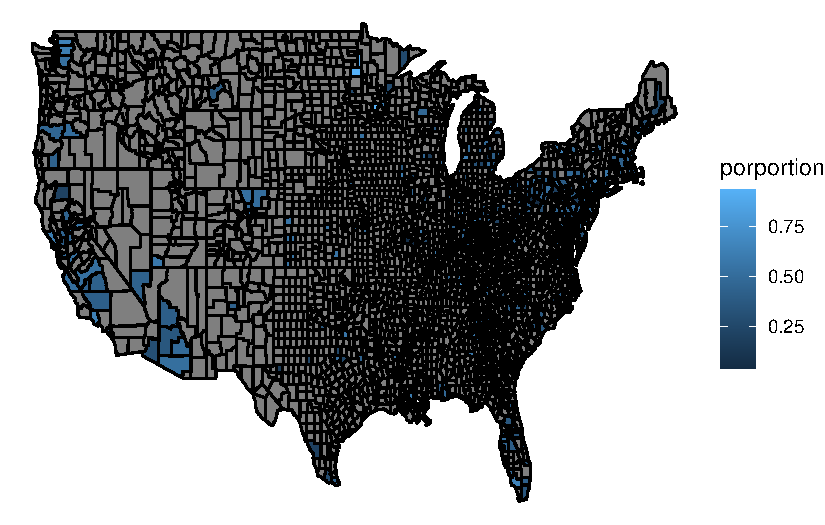
\includegraphics{GeospatialMapping_files/figure-pdf/mapping-internet-use-1.pdf}

}

\end{figure}

\begin{Shaded}
\begin{Highlighting}[]
\NormalTok{fips\_trimmed }\OtherTok{\textless{}{-}}\NormalTok{ fipsCoded }\SpecialCharTok{|\textgreater{}}
  \FunctionTok{select}\NormalTok{(fips, state, county, porportion)}

\CommentTok{\#Map for porportion of people that report using a desktop by county}
\FunctionTok{plot\_usmap}\NormalTok{(}\AttributeTok{data =}\NormalTok{ fips\_trimmed, }
           \AttributeTok{values =} \StringTok{"porportion"}\NormalTok{,}
           \AttributeTok{regions =} \StringTok{"counties"}\NormalTok{) }\SpecialCharTok{+}
  \FunctionTok{scale\_fill\_continuous}\NormalTok{(}\AttributeTok{low =} \StringTok{"white"}\NormalTok{, }\AttributeTok{high =} \StringTok{"red"}\NormalTok{, }\AttributeTok{name =} \StringTok{"Porportion of those who report using Internet"}\NormalTok{) }\SpecialCharTok{+} 
  \FunctionTok{labs}\NormalTok{(}\AttributeTok{title =} \StringTok{"County Map"}\NormalTok{)}
\end{Highlighting}
\end{Shaded}

\begin{figure}[H]

{\centering 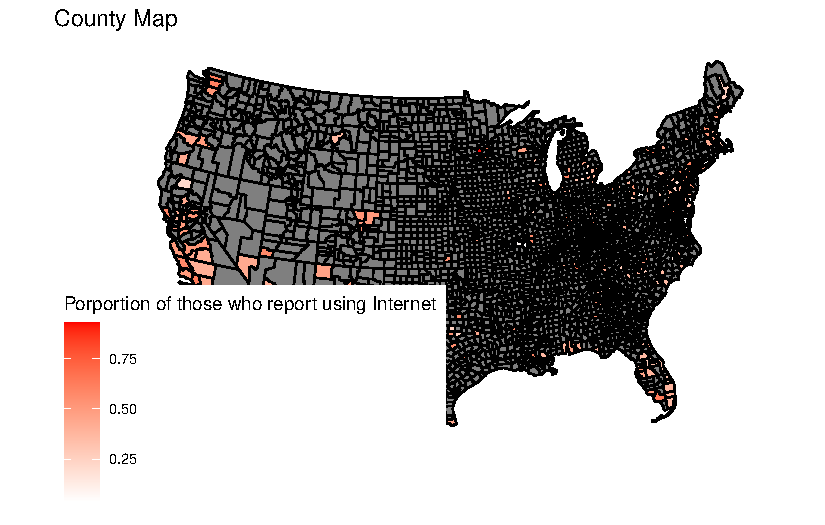
\includegraphics{GeospatialMapping_files/figure-pdf/mapping-internet-use-usmaps-package-1.pdf}

}

\end{figure}

\begin{Shaded}
\begin{Highlighting}[]
\CommentTok{\#Investigate different map packages}
\CommentTok{\#Plotting two variables on one map is difficult}
\CommentTok{\#Consider mapping two colors for reading and math scores}
\CommentTok{\#geom\_maps (maps package)}
\CommentTok{\#Dot Size + color}
\CommentTok{\#Shape + color }
\CommentTok{\#Think about the story I want to tell}
\CommentTok{\#Mapping differences between math \& reading scores}
\CommentTok{\#Think about direction of project: modeling/visualizing,deliverables, etc.}

\CommentTok{\#If I am dividing my data, note if there are differences in distributions/analysis}
\CommentTok{\#Potential mapping of district to county?}
\CommentTok{\#Stuff like the "FIPS" issues may be included in a process section, make sure to keep notes for doucmentation}
\CommentTok{\#Comparing diferent subjects, use the same scale so it\textquotesingle{}s eaiser to compare standard deivations}
\CommentTok{\#Standard deviations are good for relative comparisons and can\textquotesingle{}t be generalized to absolute values}
\CommentTok{\#See if there\textquotesingle{}s another location identifier I could use}
\CommentTok{\#Look into another long scale survey/question internet/education online/enrichment}
\CommentTok{\#Investigate the large number of not specified county codes, possibbly information not provided. See if people completed online/not specified FIPs have other geograpahic data.}
\CommentTok{\#Start bivariate }
\end{Highlighting}
\end{Shaded}

\begin{Shaded}
\begin{Highlighting}[]
\NormalTok{state\_grouped\_all }\OtherTok{\textless{}{-}}\NormalTok{ test\_state\_ys }\SpecialCharTok{|\textgreater{}}
  \FunctionTok{filter}\NormalTok{(subgroup }\SpecialCharTok{==} \StringTok{"all"}\NormalTok{) }\SpecialCharTok{|\textgreater{}}
  \FunctionTok{group\_by}\NormalTok{(sedafipsname, subject) }\SpecialCharTok{|\textgreater{}}
  \FunctionTok{summarise}\NormalTok{( }\AttributeTok{mean\_ol =} \FunctionTok{mean}\NormalTok{(ys\_mn\_2022\_ol), }\AttributeTok{mean\_eb =} \FunctionTok{mean}\NormalTok{(ys\_mn\_2022\_eb}
\NormalTok{)) }\SpecialCharTok{|\textgreater{}}
  \FunctionTok{rename}\NormalTok{ (}
    \AttributeTok{state =}\NormalTok{ sedafipsname}
\NormalTok{  )}
\end{Highlighting}
\end{Shaded}

\begin{verbatim}
`summarise()` has grouped output by 'sedafipsname'. You can override using the
`.groups` argument.
\end{verbatim}

\begin{Shaded}
\begin{Highlighting}[]
\FunctionTok{plot\_usmap}\NormalTok{(}\AttributeTok{data =}\NormalTok{ state\_grouped\_all }\SpecialCharTok{|\textgreater{}} \FunctionTok{filter}\NormalTok{(subject }\SpecialCharTok{==} \StringTok{"mth"}\NormalTok{), }\AttributeTok{values =} \StringTok{"mean\_ol"}\NormalTok{, }\AttributeTok{regions =} \StringTok{"state"}\NormalTok{) }\SpecialCharTok{+}
  \FunctionTok{scale\_fill\_continuous}\NormalTok{(}\AttributeTok{low =} \StringTok{"red"}\NormalTok{, }\AttributeTok{high =} \StringTok{"white"}\NormalTok{, }\AttributeTok{name =} \StringTok{"Test Score Difference from 2019 in standard deviations"}\NormalTok{) }\SpecialCharTok{+} 
  \FunctionTok{labs}\NormalTok{(}\AttributeTok{title =} \StringTok{"State Map"}\NormalTok{)}
\end{Highlighting}
\end{Shaded}

\begin{figure}[H]

{\centering 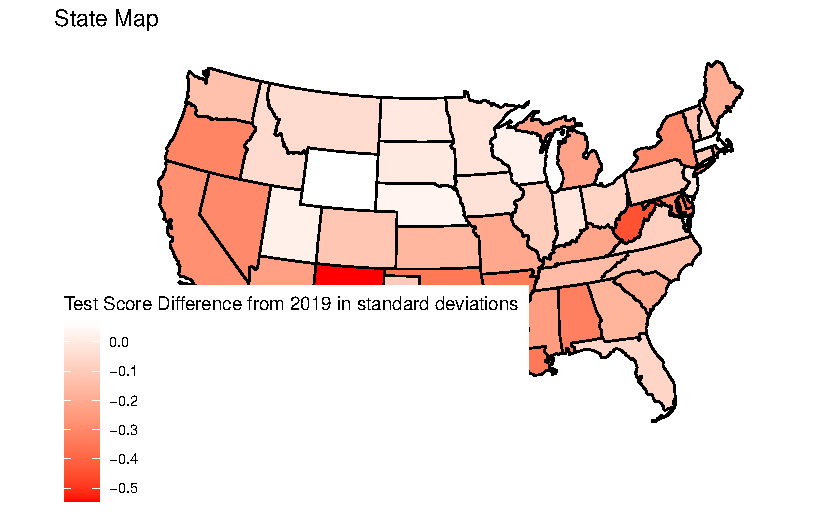
\includegraphics{GeospatialMapping_files/figure-pdf/mapping-test-scores-1.pdf}

}

\end{figure}

\begin{Shaded}
\begin{Highlighting}[]
\CommentTok{\# Neither the maps package or the USMaps package support mapping by district}
\CommentTok{\# I will try mapping districts to counties}
\CommentTok{\# https://www.census.gov/programs{-}surveys/saipe/guidance{-}geographies/districts{-}counties.html}
\CommentTok{\# If this doesn\textquotesingle{}t work out, will likely have to use the sf package with shapefiles}
\CommentTok{\# One thing }

\CommentTok{\# US Census Data on District by County}
\NormalTok{district\_by\_county }\OtherTok{\textless{}{-}} \FunctionTok{read\_excel}\NormalTok{(}\StringTok{"data/sdlist{-}21.xls"}\NormalTok{, }\AttributeTok{skip =} \DecValTok{2}\NormalTok{)}

\CommentTok{\# US Census Small Area Income and Poverty Estimates (SAIPE) by District}
\NormalTok{saipe\_district }\OtherTok{\textless{}{-}} \FunctionTok{read\_excel}\NormalTok{(}\StringTok{"data/ussd22.xls"}\NormalTok{, }\AttributeTok{skip =} \DecValTok{2}\NormalTok{)}
\end{Highlighting}
\end{Shaded}

Something to consider, sometimes states can have duplicate county names

\url{https://www.census.gov/programs-surveys/saipe/guidance-geographies/same-name/2022.html}

It is really important that I use DistrictID for each unique
\textbf{SCHOOL} district.

\begin{Shaded}
\begin{Highlighting}[]
\NormalTok{census\_clean }\OtherTok{\textless{}{-}}\NormalTok{ comp\_internet }\SpecialCharTok{|\textgreater{}}
  \FunctionTok{select}\NormalTok{(}
     \StringTok{"county\_fips"} \OtherTok{=} \StringTok{"GTCO"}\NormalTok{, }
     \StringTok{"state\_fips"} \OtherTok{=} \StringTok{"GESTFIPS"}\NormalTok{, }
     \StringTok{"Status"} \OtherTok{=} \StringTok{"HUFINAL"}\NormalTok{,}
     \StringTok{"CBSAcode"} \OtherTok{=} \StringTok{"GTCBSA"}\NormalTok{,}
     \StringTok{"UseDesktop"} \OtherTok{=} \StringTok{"HEDESKTP"}\NormalTok{, }
     \StringTok{"UseLaptop"} \OtherTok{=} \StringTok{"HELAPTOP"}\NormalTok{,  }
     \StringTok{"UseTablet"} \OtherTok{=} \StringTok{"HETABLET"}\NormalTok{,}
     \StringTok{"UseSmartphone"} \OtherTok{=} \StringTok{"HEMPHONE"}\NormalTok{,}
     \StringTok{"UseWearable"} \OtherTok{=} \StringTok{"HEWEARAB"}\NormalTok{,}
     \StringTok{"UseInternet"} \OtherTok{=} \StringTok{"HEINHOME"}\NormalTok{,}
     \StringTok{"UseInternetSchool"} \OtherTok{=} \StringTok{"HEINSCHL"}\NormalTok{, }
     \StringTok{"UseDataplan"} \OtherTok{=} \StringTok{"HEMOBDAT"}\NormalTok{,}
     \StringTok{"UseInternetTrainEdu"} \OtherTok{=} \StringTok{"PEEDTRAI"}
\NormalTok{      )}

\NormalTok{valid\_county }\OtherTok{\textless{}{-}}\NormalTok{ census\_clean }\SpecialCharTok{|\textgreater{}}
  \FunctionTok{filter}\NormalTok{(}
\NormalTok{    county\_fips }\SpecialCharTok{!=} \DecValTok{0}
\NormalTok{  ) }\SpecialCharTok{|\textgreater{}}
  \FunctionTok{mutate}\NormalTok{(}
    \AttributeTok{state =} \FunctionTok{fips\_info}\NormalTok{(state\_fips)}\SpecialCharTok{$}\NormalTok{full,}
\NormalTok{  ) }\SpecialCharTok{|\textgreater{}}
  \FunctionTok{group\_by}\NormalTok{(state, Status) }\SpecialCharTok{|\textgreater{}}
  \FunctionTok{count}\NormalTok{() }

\NormalTok{valid\_county\_sum }\OtherTok{\textless{}{-}}\NormalTok{ valid\_county }\SpecialCharTok{|\textgreater{}}
  \FunctionTok{group\_by}\NormalTok{(Status) }\SpecialCharTok{|\textgreater{}}
  \FunctionTok{summarise}\NormalTok{(}\AttributeTok{n =} \FunctionTok{sum}\NormalTok{(n)) }\SpecialCharTok{|\textgreater{}}
  \FunctionTok{arrange}\NormalTok{(}\SpecialCharTok{{-}}\NormalTok{n)}

\NormalTok{invalid\_county }\OtherTok{\textless{}{-}}\NormalTok{ census\_clean }\SpecialCharTok{|\textgreater{}}
  \FunctionTok{filter}\NormalTok{(}
\NormalTok{    county\_fips }\SpecialCharTok{==} \DecValTok{0}
\NormalTok{  ) }\SpecialCharTok{|\textgreater{}}
  \FunctionTok{mutate}\NormalTok{(}
    \AttributeTok{state =} \FunctionTok{fips\_info}\NormalTok{(state\_fips)}\SpecialCharTok{$}\NormalTok{full,}
\NormalTok{  ) }\SpecialCharTok{|\textgreater{}}
  \FunctionTok{group\_by}\NormalTok{(state, Status) }\SpecialCharTok{|\textgreater{}}
  \FunctionTok{count}\NormalTok{()}

\NormalTok{invalid\_county\_sum }\OtherTok{\textless{}{-}}\NormalTok{ invalid\_county }\SpecialCharTok{|\textgreater{}}
  \FunctionTok{group\_by}\NormalTok{(Status) }\SpecialCharTok{|\textgreater{}}
  \FunctionTok{summarise}\NormalTok{(}\AttributeTok{n =} \FunctionTok{sum}\NormalTok{(n)) }\SpecialCharTok{|\textgreater{}}
  \FunctionTok{arrange}\NormalTok{(}\SpecialCharTok{{-}}\NormalTok{n)}

\NormalTok{valid\_county\_status\_plot }\OtherTok{\textless{}{-}} \FunctionTok{ggplot}\NormalTok{(valid\_county\_sum }\SpecialCharTok{|\textgreater{}} \FunctionTok{slice}\NormalTok{(}\DecValTok{1}\SpecialCharTok{:}\DecValTok{10}\NormalTok{)) }\SpecialCharTok{+}
  \FunctionTok{geom\_col}\NormalTok{(}\FunctionTok{aes}\NormalTok{(}\AttributeTok{x =} \FunctionTok{reorder}\NormalTok{(Status, }\SpecialCharTok{{-}}\NormalTok{n), }\AttributeTok{y =}\NormalTok{ n) ) }\SpecialCharTok{+}
  \CommentTok{\#geom\_col(data = invalid\_county\_sum) +}
  \FunctionTok{labs}\NormalTok{(}
    \AttributeTok{title =} \StringTok{"Distribution of Codes"}\NormalTok{,}
    \AttributeTok{subtitle =} \StringTok{"Among Responses with Valid counties"}
\NormalTok{  ) }\SpecialCharTok{+}
  \FunctionTok{scale\_y\_continuous}\NormalTok{( }\AttributeTok{limits =} \FunctionTok{c}\NormalTok{(}\DecValTok{0}\NormalTok{, }\DecValTok{60000}\NormalTok{) )}

\NormalTok{invalid\_county\_status\_plot }\OtherTok{\textless{}{-}} \FunctionTok{ggplot}\NormalTok{(invalid\_county\_sum }\SpecialCharTok{|\textgreater{}} \FunctionTok{slice}\NormalTok{(}\DecValTok{1}\SpecialCharTok{:}\DecValTok{10}\NormalTok{)) }\SpecialCharTok{+}
  \FunctionTok{geom\_col}\NormalTok{(}\FunctionTok{aes}\NormalTok{(}\AttributeTok{x =} \FunctionTok{reorder}\NormalTok{(Status, }\SpecialCharTok{{-}}\NormalTok{n), }\AttributeTok{y =}\NormalTok{ n)) }\SpecialCharTok{+}
  \FunctionTok{labs}\NormalTok{(}
    \AttributeTok{title =} \StringTok{"Distribution of codes"}\NormalTok{,}
    \AttributeTok{subtitle =} \StringTok{"Among Responses with Invalid counties"}
\NormalTok{  ) }\SpecialCharTok{+}
  \FunctionTok{scale\_y\_continuous}\NormalTok{( }\AttributeTok{limits =} \FunctionTok{c}\NormalTok{(}\DecValTok{0}\NormalTok{, }\DecValTok{60000}\NormalTok{) )}

\NormalTok{valid\_county\_status\_plot }\SpecialCharTok{+}\NormalTok{ invalid\_county\_status\_plot}
\end{Highlighting}
\end{Shaded}

\begin{figure}[H]

{\centering 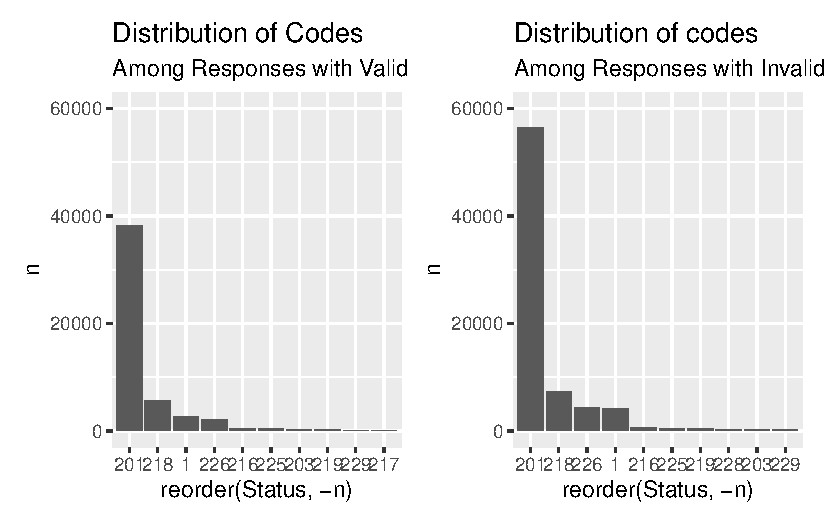
\includegraphics{GeospatialMapping_files/figure-pdf/looking-into-missing-county-data-1.pdf}

}

\end{figure}

There does not appear to be a significant difference in the completion
code distribution between respondents in valid counties vs invalid
counties

Code Mappings for ``Status''

1: Fully Complete CATI (computer-assisted telephone interviewing)

2: Partially Complete CATI

201: CAPI (computer-assisted personal interviewing)

There appears to be no correlation between the interview completion

\begin{Shaded}
\begin{Highlighting}[]
\CommentTok{\#Mapping by state since county data is very incomplete}
\NormalTok{comp\_state\_mapping }\OtherTok{\textless{}{-}}\NormalTok{ comp\_internet }\SpecialCharTok{|\textgreater{}}
  \FunctionTok{select}\NormalTok{(}
     \StringTok{"county\_fips"} \OtherTok{=} \StringTok{"GTCO"}\NormalTok{, }
     \StringTok{"Status"} \OtherTok{=} \StringTok{"HUFINAL"}\NormalTok{,}
     \StringTok{"state\_fips"} \OtherTok{=} \StringTok{"GESTFIPS"}\NormalTok{, }
     \StringTok{"CBSAcode"} \OtherTok{=} \StringTok{"GTCBSA"}\NormalTok{,}
     \StringTok{"UseDesktop"} \OtherTok{=} \StringTok{"HEDESKTP"}\NormalTok{, }
     \StringTok{"UseLaptop"} \OtherTok{=} \StringTok{"HELAPTOP"}\NormalTok{,  }
     \StringTok{"UseTablet"} \OtherTok{=} \StringTok{"HETABLET"}\NormalTok{,}
     \StringTok{"UseSmartphone"} \OtherTok{=} \StringTok{"HEMPHONE"}\NormalTok{,}
     \StringTok{"UseWearable"} \OtherTok{=} \StringTok{"HEWEARAB"}\NormalTok{,}
     \StringTok{"UseInternet"} \OtherTok{=} \StringTok{"HEINHOME"}\NormalTok{,}
     \StringTok{"UseInternetSchool"} \OtherTok{=} \StringTok{"HEINSCHL"}\NormalTok{, }
     \StringTok{"UseDataplan"} \OtherTok{=} \StringTok{"HEMOBDAT"}\NormalTok{,}
     \StringTok{"UseInternetTrainEdu"} \OtherTok{=} \StringTok{"PEEDTRAI"}
\NormalTok{      ) }\SpecialCharTok{|\textgreater{}}
  \FunctionTok{drop\_na}\NormalTok{(state\_fips, county\_fips) }\SpecialCharTok{|\textgreater{}}
  \FunctionTok{filter}\NormalTok{(}
    \FunctionTok{any}\NormalTok{(Status }\SpecialCharTok{==}\NormalTok{ complete\_codes)}
\NormalTok{  ) }\SpecialCharTok{|\textgreater{}}
  \FunctionTok{mutate}\NormalTok{(}
    \AttributeTok{state =} \FunctionTok{fips\_info}\NormalTok{(state\_fips)}\SpecialCharTok{$}\NormalTok{full}
\NormalTok{  ) }\SpecialCharTok{|\textgreater{}}
  \FunctionTok{group\_by}\NormalTok{(state, UseDesktop) }\SpecialCharTok{|\textgreater{}}
  \FunctionTok{count}\NormalTok{() }\SpecialCharTok{|\textgreater{}}
  \FunctionTok{filter}\NormalTok{(UseDesktop }\SpecialCharTok{==} \DecValTok{1} \SpecialCharTok{|}\NormalTok{ UseDesktop }\SpecialCharTok{==} \DecValTok{2}\NormalTok{) }\SpecialCharTok{|\textgreater{}}
  \FunctionTok{pivot\_wider}\NormalTok{(}
    \AttributeTok{names\_from =}\NormalTok{ UseDesktop,}
    \AttributeTok{values\_from =}\NormalTok{ n}
\NormalTok{  ) }\SpecialCharTok{|\textgreater{}}
  \FunctionTok{rename}\NormalTok{( }\AttributeTok{Yes =} \StringTok{"1"}\NormalTok{, }\AttributeTok{No =} \StringTok{"2"}\NormalTok{ ) }\SpecialCharTok{|\textgreater{}}
  \FunctionTok{mutate}\NormalTok{(}\AttributeTok{porportion =}\NormalTok{ Yes}\SpecialCharTok{/}\NormalTok{(Yes }\SpecialCharTok{+}\NormalTok{ No))}

\NormalTok{state\_map }\OtherTok{\textless{}{-}} \FunctionTok{map\_data}\NormalTok{(}\StringTok{"state"}\NormalTok{) }\SpecialCharTok{|\textgreater{}}
  \FunctionTok{mutate}\NormalTok{(}
  \StringTok{"region"} \OtherTok{=} \FunctionTok{str\_to\_title}\NormalTok{(region),}
\NormalTok{  ) }

\NormalTok{internet\_map }\OtherTok{\textless{}{-}}\NormalTok{ comp\_state\_mapping }\SpecialCharTok{|\textgreater{}}
  \FunctionTok{left\_join}\NormalTok{(state\_map, }\AttributeTok{by =} \FunctionTok{join\_by}\NormalTok{(state }\SpecialCharTok{==}\NormalTok{ region))}

\NormalTok{state\_centroids }\OtherTok{\textless{}{-}}\NormalTok{ state\_map}\SpecialCharTok{|\textgreater{}}
  \FunctionTok{group\_by}\NormalTok{(region) }\SpecialCharTok{|\textgreater{}}
  \FunctionTok{summarise}\NormalTok{( }\AttributeTok{long =} \FunctionTok{mean}\NormalTok{ (long), }\AttributeTok{lat =} \FunctionTok{mean}\NormalTok{(lat))}

\NormalTok{score\_map }\OtherTok{\textless{}{-}}\NormalTok{ state\_grouped\_all }\SpecialCharTok{|\textgreater{}}
  \FunctionTok{left\_join}\NormalTok{(state\_centroids, }\AttributeTok{by =} \FunctionTok{join\_by}\NormalTok{(state }\SpecialCharTok{==}\NormalTok{ region))}


\FunctionTok{ggplot}\NormalTok{(internet\_map, }\FunctionTok{aes}\NormalTok{(}\AttributeTok{x =}\NormalTok{ long, }\AttributeTok{y =}\NormalTok{ lat)) }\SpecialCharTok{+}
    \FunctionTok{geom\_polygon}\NormalTok{(}\FunctionTok{aes}\NormalTok{(}\AttributeTok{group =}\NormalTok{ group, }\AttributeTok{fill =}\NormalTok{ porportion), }\AttributeTok{color =} \StringTok{"black"}\NormalTok{) }\SpecialCharTok{+}
    \FunctionTok{geom\_point}\NormalTok{(}\AttributeTok{data =}\NormalTok{ score\_map, }\AttributeTok{size =} \DecValTok{4}\NormalTok{, }\FunctionTok{aes}\NormalTok{(}\AttributeTok{color =}\NormalTok{ mean\_ol)) }\SpecialCharTok{+}
    \FunctionTok{scale\_color\_viridis\_c}\NormalTok{(}\AttributeTok{option =} \StringTok{"A"}\NormalTok{) }\SpecialCharTok{+}
    \FunctionTok{theme\_void}\NormalTok{() }\SpecialCharTok{+}
    \FunctionTok{labs}\NormalTok{(}
      \AttributeTok{fill =} \StringTok{"Porportion of Reported}\SpecialCharTok{\textbackslash{}n}\StringTok{Internet Usage"}
\NormalTok{    )}
\end{Highlighting}
\end{Shaded}

\begin{verbatim}
Warning: Removed 4 rows containing missing values (`geom_point()`).
\end{verbatim}

\begin{figure}[H]

{\centering 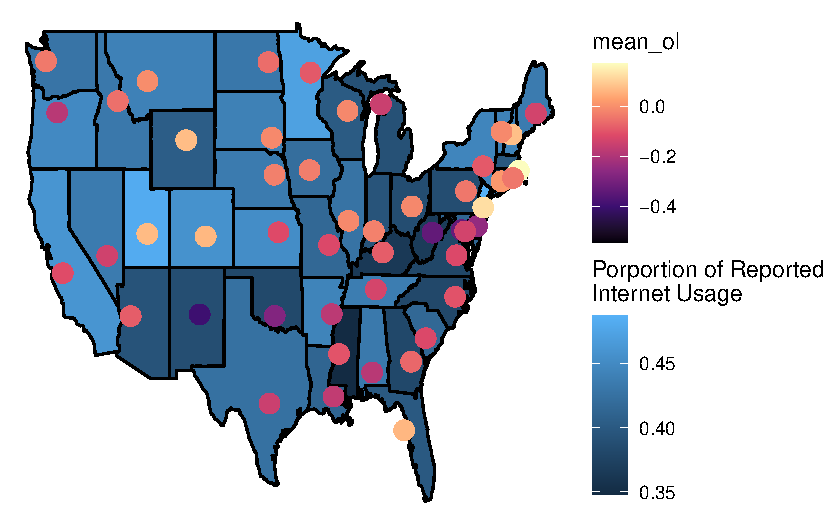
\includegraphics{GeospatialMapping_files/figure-pdf/bivariate-mapping-1.pdf}

}

\end{figure}

Unfortunately, it's really hard to make meaningful conclusions or
analysis about state metrics

\begin{Shaded}
\begin{Highlighting}[]
\CommentTok{\#Since county codes did not cover a significant geographic portion of the US, I want to see if CBSA codes could provide better coverage}

\CommentTok{\#Show distribution of country codes}
\NormalTok{comp\_internet }\SpecialCharTok{|\textgreater{}}
  \FunctionTok{group\_by}\NormalTok{(GTCO) }\SpecialCharTok{|\textgreater{}}
  \FunctionTok{summarise}\NormalTok{( }\AttributeTok{count =} \FunctionTok{n}\NormalTok{())}
\end{Highlighting}
\end{Shaded}

\begin{verbatim}
# A tibble: 100 x 2
    GTCO count
   <dbl> <int>
 1     0 76179
 2     1  4441
 3     3  4385
 4     5  1690
 5     7   281
 6     9   797
 7    11  1262
 8    13  2380
 9    15   611
10    17  1362
# i 90 more rows
\end{verbatim}

\begin{Shaded}
\begin{Highlighting}[]
\CommentTok{\#Show how manny nonzero country codes there were}
\NormalTok{comp\_internet }\SpecialCharTok{|\textgreater{}}
  \FunctionTok{filter}\NormalTok{(GTCO }\SpecialCharTok{!=} \DecValTok{0}\NormalTok{) }\SpecialCharTok{|\textgreater{}}
  \FunctionTok{summarise}\NormalTok{( }\AttributeTok{count =} \FunctionTok{n}\NormalTok{())}
\end{Highlighting}
\end{Shaded}

\begin{verbatim}
# A tibble: 1 x 1
  count
  <int>
1 51196
\end{verbatim}

\begin{Shaded}
\begin{Highlighting}[]
\CommentTok{\#Distribution of CBSA codes}
\NormalTok{comp\_internet }\SpecialCharTok{|\textgreater{}}
  \FunctionTok{group\_by}\NormalTok{(GTCBSA) }\SpecialCharTok{|\textgreater{}}
  \FunctionTok{count}\NormalTok{() }\SpecialCharTok{|\textgreater{}}
  \FunctionTok{arrange}\NormalTok{(}\SpecialCharTok{{-}}\NormalTok{n)}
\end{Highlighting}
\end{Shaded}

\begin{verbatim}
# A tibble: 261 x 2
# Groups:   GTCBSA [261]
   GTCBSA     n
    <dbl> <int>
 1      0 33615
 2  35620  5025
 3  47900  3815
 4  31080  3464
 5  16980  2516
 6  37980  2283
 7  14460  2189
 8  19100  2010
 9  26420  1888
10  33100  1525
# i 251 more rows
\end{verbatim}

\begin{Shaded}
\begin{Highlighting}[]
\CommentTok{\#Show how many nonzero CBSA codes}
\NormalTok{comp\_internet }\SpecialCharTok{|\textgreater{}}
  \FunctionTok{filter}\NormalTok{(GTCBSA }\SpecialCharTok{!=} \DecValTok{0}\NormalTok{) }\SpecialCharTok{|\textgreater{}}
  \FunctionTok{count}\NormalTok{()}
\end{Highlighting}
\end{Shaded}

\begin{verbatim}
# A tibble: 1 x 1
      n
  <int>
1 93760
\end{verbatim}

In conclusion, while there are fewer invalid/incomplete CBSA codes, a
vast majority of other datasets tend to use districts or counties. As
such, I will not be moving forward with CBSA codes.

The Educational Opportunity Project Standardizes their data with the
Stanford Education Data Archive (SEDA). They created their own
identifier for each district,
\texttt{SEDA\ Administrative\ District\ ID}, which details can be found
here: \url{https://edopportunity.org/methods/}

\begin{Shaded}
\begin{Highlighting}[]
\NormalTok{test\_admindist\_gys }\OtherTok{\textless{}{-}}\NormalTok{ test\_admindist\_gys }\SpecialCharTok{|\textgreater{}}
  \FunctionTok{mutate}\NormalTok{(}
    \AttributeTok{diff22\_23 =}\NormalTok{ gys\_mn\_2023\_ol }\SpecialCharTok{{-}}\NormalTok{ gys\_mn\_2022\_ol}
\NormalTok{  )}

\FunctionTok{ggplot}\NormalTok{(test\_admindist\_gys) }\SpecialCharTok{+}
  \FunctionTok{geom\_jitter}\NormalTok{(}
    \FunctionTok{aes}\NormalTok{(}
      \AttributeTok{x =}\NormalTok{ subgroup,}
      \AttributeTok{y =}\NormalTok{ gys\_mn\_2022\_ol,}
      \AttributeTok{color =}\NormalTok{ gys\_mn\_2022\_ol}
\NormalTok{      ),}
\NormalTok{    ) }\SpecialCharTok{+}
  \FunctionTok{facet\_grid}\NormalTok{(}
    \AttributeTok{cols =} \FunctionTok{vars}\NormalTok{(subject)}
\NormalTok{  )}
\end{Highlighting}
\end{Shaded}

\begin{figure}[H]

{\centering 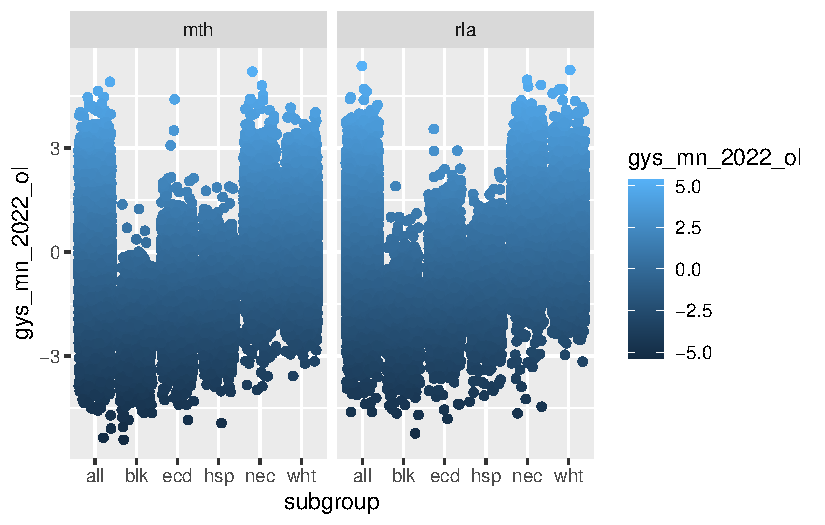
\includegraphics{GeospatialMapping_files/figure-pdf/district-scores-scatter-1.pdf}

}

\end{figure}

\begin{Shaded}
\begin{Highlighting}[]
\FunctionTok{ggplot}\NormalTok{(test\_admindist\_gys) }\SpecialCharTok{+}
  \FunctionTok{geom\_jitter}\NormalTok{(}
    \FunctionTok{aes}\NormalTok{(}
      \AttributeTok{x =}\NormalTok{ subgroup,}
      \AttributeTok{y =}\NormalTok{ gys\_mn\_2023\_ol,}
      \AttributeTok{color =}\NormalTok{ gys\_mn\_2023\_ol}
\NormalTok{      ),}
\NormalTok{    ) }\SpecialCharTok{+}
  \FunctionTok{facet\_grid}\NormalTok{(}
    \AttributeTok{cols =} \FunctionTok{vars}\NormalTok{(subject)}
\NormalTok{  ) }
\end{Highlighting}
\end{Shaded}

\begin{verbatim}
Warning: Removed 9374 rows containing missing values (`geom_point()`).
\end{verbatim}

\begin{figure}[H]

{\centering 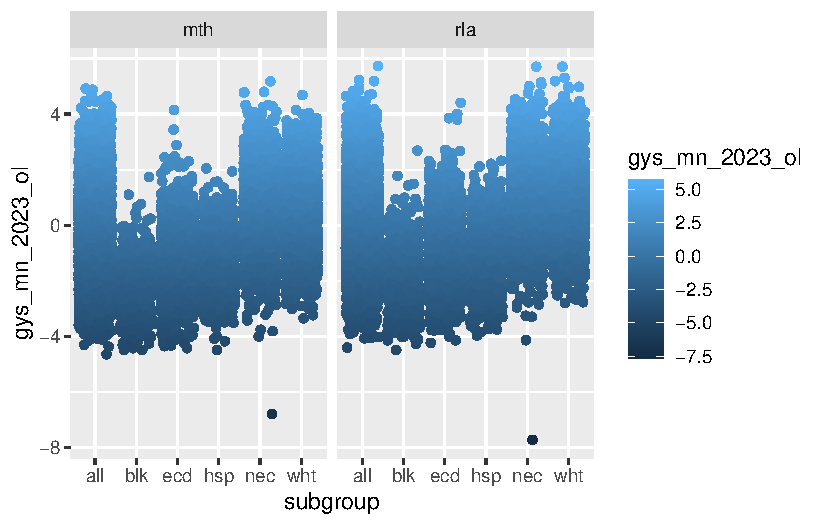
\includegraphics{GeospatialMapping_files/figure-pdf/district-scores-scatter-2.pdf}

}

\end{figure}

\begin{Shaded}
\begin{Highlighting}[]
\FunctionTok{ggplot}\NormalTok{(test\_admindist\_gys }\SpecialCharTok{|\textgreater{}} \FunctionTok{filter}\NormalTok{ (subject }\SpecialCharTok{==} \StringTok{"mth"}\NormalTok{)) }\SpecialCharTok{+}
  \FunctionTok{geom\_jitter}\NormalTok{(}
    \FunctionTok{aes}\NormalTok{(}
      \AttributeTok{x =}\NormalTok{ subgroup,}
      \AttributeTok{y =}\NormalTok{ gys\_mn\_2022\_ol,}
      \AttributeTok{color =}\NormalTok{ gys\_mn\_2022\_ol}
\NormalTok{      ),}
\NormalTok{    ) }\SpecialCharTok{+}
  \FunctionTok{scale\_y\_continuous}\NormalTok{(}
    \AttributeTok{limits =} \FunctionTok{c}\NormalTok{(}\SpecialCharTok{{-}}\DecValTok{6}\NormalTok{, }\DecValTok{6}\NormalTok{)}
\NormalTok{  ) }\SpecialCharTok{+}

\FunctionTok{ggplot}\NormalTok{(test\_admindist\_gys }\SpecialCharTok{|\textgreater{}} \FunctionTok{filter}\NormalTok{ (subject }\SpecialCharTok{==} \StringTok{"mth"}\NormalTok{)) }\SpecialCharTok{+}
  \FunctionTok{geom\_jitter}\NormalTok{(}
    \FunctionTok{aes}\NormalTok{(}
      \AttributeTok{x =}\NormalTok{ subgroup,}
      \AttributeTok{y =}\NormalTok{ gys\_mn\_2023\_ol,}
      \AttributeTok{color =}\NormalTok{ gys\_mn\_2023\_ol}
\NormalTok{      ),}
\NormalTok{    ) }\SpecialCharTok{+}
  \FunctionTok{scale\_y\_continuous}\NormalTok{(}
    \AttributeTok{limits =} \FunctionTok{c}\NormalTok{(}\SpecialCharTok{{-}}\DecValTok{6}\NormalTok{, }\DecValTok{6}\NormalTok{)}
\NormalTok{  )}
\end{Highlighting}
\end{Shaded}

\begin{verbatim}
Warning: Removed 4959 rows containing missing values (`geom_point()`).
\end{verbatim}

\begin{figure}[H]

{\centering 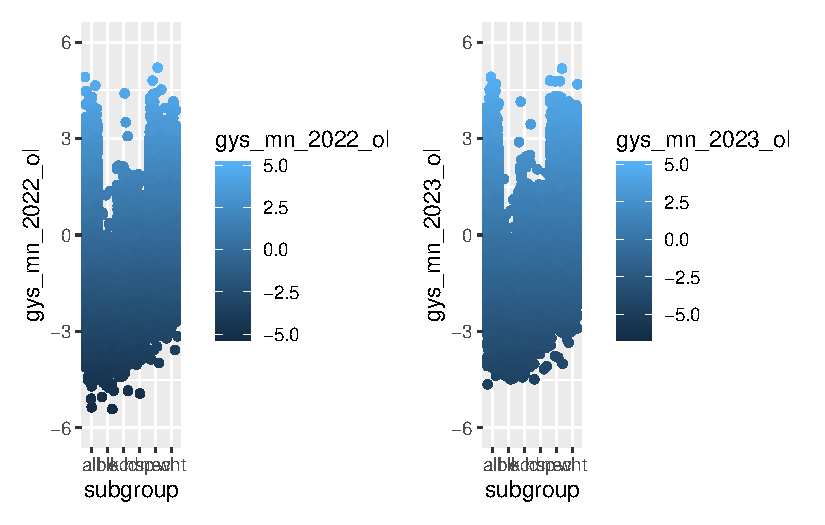
\includegraphics{GeospatialMapping_files/figure-pdf/district-scores-scatter-3.pdf}

}

\end{figure}

\begin{Shaded}
\begin{Highlighting}[]
\FunctionTok{ggplot}\NormalTok{(test\_admindist\_gys}\SpecialCharTok{|\textgreater{}} \FunctionTok{filter}\NormalTok{ (subject }\SpecialCharTok{==} \StringTok{"mth"}\NormalTok{, subgroup }\SpecialCharTok{==} \StringTok{"all"}\NormalTok{)) }\SpecialCharTok{+}
  \FunctionTok{geom\_jitter}\NormalTok{(}
    \FunctionTok{aes}\NormalTok{(}
      \AttributeTok{x =} \DecValTok{0}\NormalTok{,}
      \AttributeTok{y =}\NormalTok{ diff22\_23,}
      \AttributeTok{color =}\NormalTok{ diff22\_23,}
\NormalTok{      ),}
\NormalTok{    ) }\SpecialCharTok{+}
  \FunctionTok{scale\_x\_continuous}\NormalTok{(}\AttributeTok{limits =} \FunctionTok{c}\NormalTok{(}\SpecialCharTok{{-}}\DecValTok{1}\NormalTok{,}\DecValTok{1}\NormalTok{)) }\SpecialCharTok{+}
  \FunctionTok{scale\_color\_viridis\_c}\NormalTok{()}
\end{Highlighting}
\end{Shaded}

\begin{verbatim}
Warning: Removed 1463 rows containing missing values (`geom_point()`).
\end{verbatim}

\begin{figure}[H]

{\centering 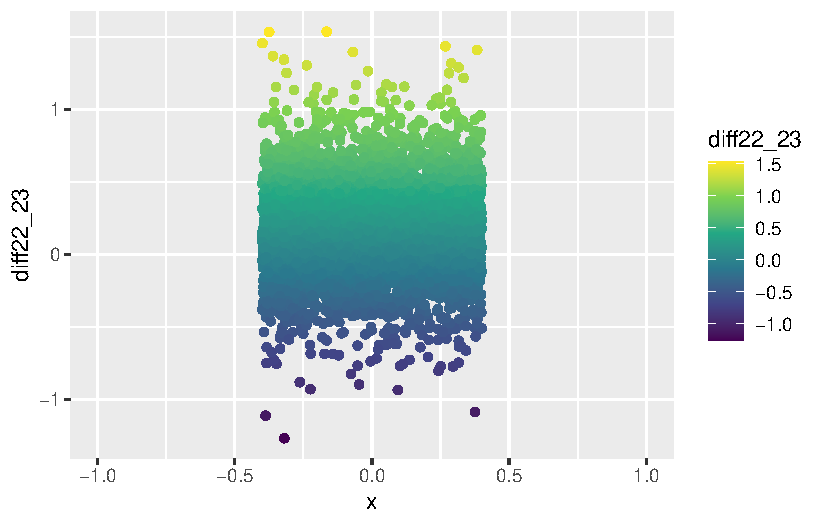
\includegraphics{GeospatialMapping_files/figure-pdf/district-scores-scatter-4.pdf}

}

\end{figure}

\begin{Shaded}
\begin{Highlighting}[]
\FunctionTok{mean}\NormalTok{(}\FunctionTok{na.omit}\NormalTok{(test\_admindist\_gys}\SpecialCharTok{$}\NormalTok{gys\_mn\_2022\_ol))}
\end{Highlighting}
\end{Shaded}

\begin{verbatim}
[1] -0.2498951
\end{verbatim}

\begin{Shaded}
\begin{Highlighting}[]
\FunctionTok{median}\NormalTok{(}\FunctionTok{na.omit}\NormalTok{(test\_admindist\_gys}\SpecialCharTok{$}\NormalTok{gys\_mn\_2022\_ol))}
\end{Highlighting}
\end{Shaded}

\begin{verbatim}
[1] -0.2672775
\end{verbatim}

\begin{Shaded}
\begin{Highlighting}[]
\FunctionTok{median}\NormalTok{(}\FunctionTok{na.omit}\NormalTok{(test\_admindist\_gys}\SpecialCharTok{$}\NormalTok{gys\_mn\_2023\_ol))}
\end{Highlighting}
\end{Shaded}

\begin{verbatim}
[1] -0.0795574
\end{verbatim}

\begin{Shaded}
\begin{Highlighting}[]
\FunctionTok{ggplot}\NormalTok{(test\_admindist\_gys) }\SpecialCharTok{+}
  \FunctionTok{geom\_density}\NormalTok{(}
    \FunctionTok{aes}\NormalTok{(}
      \AttributeTok{x =}\NormalTok{ gys\_mn\_2022\_ol,}
\NormalTok{      ),}
    \AttributeTok{fill =} \StringTok{"orange"}
\NormalTok{  )}
\end{Highlighting}
\end{Shaded}

\begin{figure}[H]

{\centering 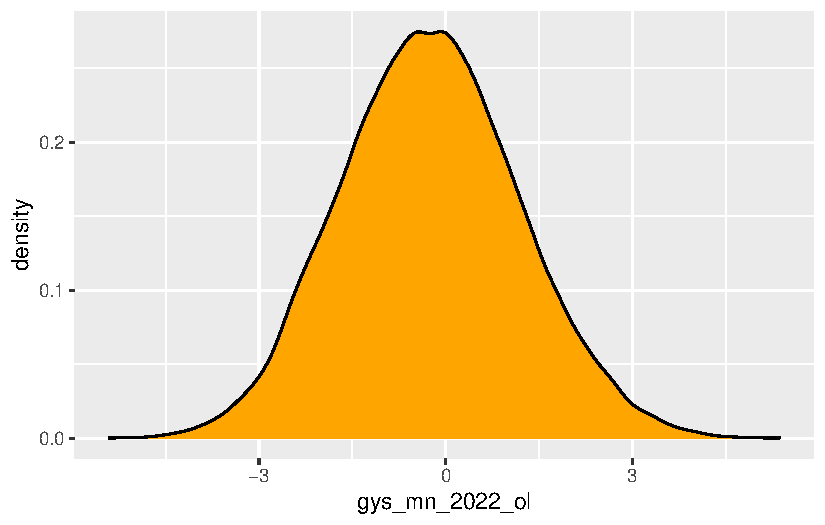
\includegraphics{GeospatialMapping_files/figure-pdf/district-scores-density-1.pdf}

}

\end{figure}

\begin{Shaded}
\begin{Highlighting}[]
\FunctionTok{ggplot}\NormalTok{(test\_admindist\_gys) }\SpecialCharTok{+}
  \FunctionTok{geom\_density}\NormalTok{(}
    \FunctionTok{aes}\NormalTok{(}
      \AttributeTok{x =}\NormalTok{ gys\_mn\_2023\_ol,}
\NormalTok{      ),}
    \AttributeTok{fill =} \StringTok{"orange"}
\NormalTok{  )}
\end{Highlighting}
\end{Shaded}

\begin{verbatim}
Warning: Removed 9374 rows containing non-finite values (`stat_density()`).
\end{verbatim}

\begin{figure}[H]

{\centering 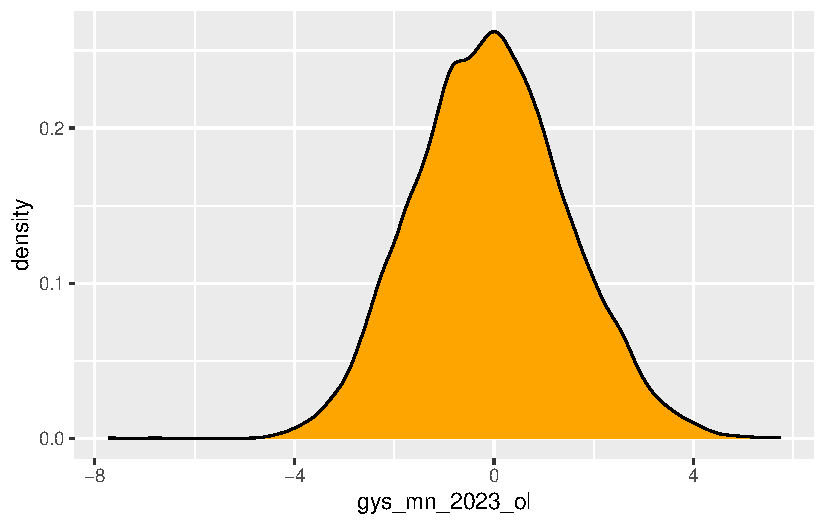
\includegraphics{GeospatialMapping_files/figure-pdf/district-scores-density-2.pdf}

}

\end{figure}

\begin{Shaded}
\begin{Highlighting}[]
\FunctionTok{ggplot}\NormalTok{(test\_admindist\_gys) }\SpecialCharTok{+}
  \FunctionTok{geom\_density}\NormalTok{(}
    \FunctionTok{aes}\NormalTok{(}
      \AttributeTok{x =}\NormalTok{ diff22\_23,}
\NormalTok{      ),}
    \AttributeTok{fill =} \StringTok{"orange"}
\NormalTok{  )}
\end{Highlighting}
\end{Shaded}

\begin{verbatim}
Warning: Removed 9374 rows containing non-finite values (`stat_density()`).
\end{verbatim}

\begin{figure}[H]

{\centering 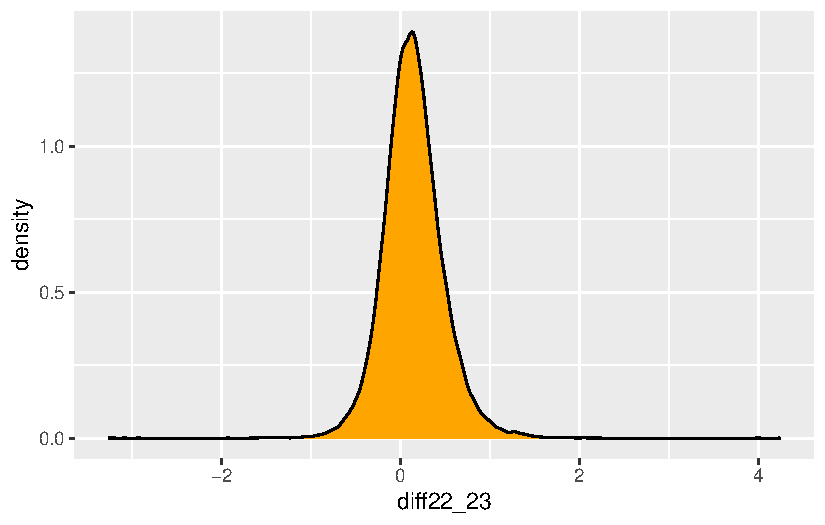
\includegraphics{GeospatialMapping_files/figure-pdf/district-scores-density-3.pdf}

}

\end{figure}

\hypertarget{more-resources-to-consider}{%
\paragraph{More Resources to
Consider}\label{more-resources-to-consider}}

Additional Census Data:

\begin{itemize}
\item
  Household income in the past year\\
  \url{https://data.census.gov/table/ACSST1Y2021.S2503?t=Financial\%20Characteristics\&g=010XX00US$0500000\&y=2021\&tp=true}
\item
  Age + Race Demographics\\
  \url{https://data.census.gov/table/ACSDP1Y2021.DP05?g=010XX00US$0500000\&y=2021\&tp=true}
\item
  Characteristics of Foreign Born Population\\
  \url{https://data.census.gov/table/ACSST1Y2021.S0501?g=010XX00US$0500000\&y=2021\&tp=true}
\end{itemize}

School Budget/School Opening/State Funding

\url{https://about.burbio.com/\#sign-up}

Absenteeism

\url{https://www.future-ed.org/tracking-state-trends-in-chronic-absenteeism/}

Additional Metrics

\begin{itemize}
\item
  Literacy/Active Reading in Households
\item
  Education level of parents/family

  \begin{itemize}
  \tightlist
  \item
    Bachelor's \%
  \end{itemize}
\item
  General COVID statistics (cases, deaths, etc.)
\item
  Recovery Strategies

  \begin{itemize}
  \tightlist
  \item
    Look into outliers in the trends and what they are doing
  \end{itemize}
\item
  Inner-district disparities among schools
\end{itemize}

Referenced Reports/Resources

\begin{itemize}
\item
  \url{https://www.nytimes.com/interactive/2024/01/31/us/pandemic-learning-loss-recovery.html}
\item
  \href{https://www.nytimes.com/interactive/2024/02/01/upshot/learning-loss-school-districts.html?searchResultPosition=10}{https://www.nytimes.com/interactive/2024/02/01/upshot/learning-loss-school-districts.html}
\item
  \url{https://www.nytimes.com/2023/12/09/opinion/education-learning-loss.html}
\item
  \url{https://www.nytimes.com/2023/11/17/us/chronic-absenteeism-pandemic-recovery.html}
\item
  \url{https://educationrecoveryscorecard.org/}
\item
  \url{https://edopportunity.org/}
\end{itemize}

General Plan:

\begin{itemize}
\item
  How to handle changing districts

  \begin{itemize}
  \item
    Look into other reports
  \item
    Census website
  \item
    Maybe just pick a specific year
  \item
    Take aggregate measurement over time periods
  \item
    Possibly look at the data across years and determine if there's
    enough variability
  \end{itemize}
\item
  Main Visualization:

  \begin{itemize}
  \item
    Scatterplot (based on \url{https://educationrecoveryscorecard.org/})

    \begin{itemize}
    \item
      Y: Reading/Math Scores
    \item
      X: Some metric
    \item
      Filters: other metrics (location, income, race, etc.)
    \end{itemize}
  \item
    Scatterplot

    \begin{itemize}
    \item
      Y: Reading Score
    \item
      X: Math score
    \item
      Filters: metrics
    \end{itemize}
  \end{itemize}
\item
  Look into district level data

  \begin{itemize}
  \item
    What data the project uses

    \begin{itemize}
    \item
      \url{https://edopportunity.org/help-faq/\#how-is-ses}
    \item
      For socioeconomic status, they use data from the American
      Community Survey (found on data.census.gov)
    \item
      data/ACS\_SchoolDistricts\_Socioeconomic\_2021/ACSDP1Y2021.DP04-Data.csv

      \begin{itemize}
      \item
        Monthly Owner Costs
      \item
        Monthly Owner Costs as percentage of household income
      \item
        Owner-occupied units value
      \end{itemize}
    \end{itemize}
  \item
    Their methodology

    \begin{itemize}
    \tightlist
    \item
      \url{https://edopportunity.org/docs/seda2023_documentation_20240130.pdf}
    \end{itemize}
  \item
    How I can merge in outside datasets

    \begin{itemize}
    \tightlist
    \item
      Census datasets have data per school district
    \end{itemize}
  \end{itemize}
\item
  Percent of counties with multiple districts

  \begin{itemize}
  \tightlist
  \item
    Determines how important it is to get district level data
  \end{itemize}
\item
  SEDA Technical Document

  \begin{itemize}
  \item
    What is a SEDA Administrative District?

    \begin{itemize}
    \item
      In 4.1, they used geographic districts

      \begin{itemize}
      \tightlist
      \item
        If you had magnet/charter schools, it could have been operated
        in district A but managed by district B
      \end{itemize}
    \item
      In 5.0, they are using administrative districts

      \begin{itemize}
      \tightlist
      \item
        An administrative districts represents all schools that are
        managed by the district
      \end{itemize}
    \end{itemize}
  \item
    Should be really easy to map SEDA Admin district to ACS School
    District
  \end{itemize}
\item
  Mapping in Shiny

  \begin{itemize}
  \item
    Hard to avoid re-rendering the map every time a selection is changed

    \begin{itemize}
    \tightlist
    \item
      side note: maybe find a way to reduce render time
    \end{itemize}
  \item
    Maps package options: (sf, usmaps, maps, leaflet)

    \begin{itemize}
    \item
      sf: Probably the most robust and customizable

      \begin{itemize}
      \tightlist
      \item
        I can get shapefiles from government websites for school
        districts
      \end{itemize}
    \item
      usmaps: More intuitive to use, but lack of division options
    \item
      maps: Less intuitive
    \item
      leaflet: More functionality (zoom, pre-rendering)
    \end{itemize}
  \end{itemize}
\item
  Scatterplot in Shiny

  \begin{itemize}
  \item
    Look into hovering/clicking functionality for plotted points

    \begin{itemize}
    \tightlist
    \item
      Be able to register that a click occurred and where
    \end{itemize}
  \end{itemize}
\item
  Todo:

  \begin{itemize}
  \item
    Data Joining (ACS to Academic Performance)

    \begin{itemize}
    \item
      If any issues, try to find quick fixes
    \item
      Even if there issues, keep moving forward
    \end{itemize}
  \item
    Create the scatterplot comparing some socioeconomic metric (x) to
    reading/math scores (y)

    \begin{itemize}
    \tightlist
    \item
      Include other aesthetics once the point distribution is good
    \end{itemize}
  \item
    Create antoher scatterplot that compares reading score (x) to math
    score (y)

    \begin{itemize}
    \tightlist
    \item
      Try to put in additional aesthetics (socioeconomic)
    \end{itemize}
  \item
    Start working on the app

    \begin{itemize}
    \tightlist
    \item
      Put one of my nice plots into the app
    \end{itemize}
  \end{itemize}
\end{itemize}



\end{document}
